\documentclass[letterpaper, 12pt]{article}
\usepackage{fullpage}
\usepackage{cite}
\usepackage{graphicx}
\graphicspath{ {images/} }

\begin{document}

\title{Graph Isomorphism}
\author{Franklin van Nes}
\date{Tuesday 12th November, 2017}
\maketitle


    Graph Isomorphism is most intuitively understood through its greek etymology: \textit{Iso}, meaning
     same, and \textit{morphism}, meaning shape; \textit{Graph Isomorhpism} $\rightarrow$ graphs that share the same shape.
    In more detail, two finite graphs are isomorphic if they share the same number of vertices connected in the same way.
    \\\\
    Formally, by an \textit{isomorphism} we mean from two graphs $G_1$ to $G_2$ we have a one-to-one mapping $f: G_1.V \rightarrow G_2.V$ from $G_1.V$ onto $G_2.V$ so
    that vertices $u_1$ and $v_1$ are adjacent in $G_1$ if and only if the vertices $f(u_1)$ and $f(v_1)$ are adjacent in $G_2$.
    If an isomorphism exists between $G_1$ and $G_2$, we say they are \textit{isomorphic}~\cite{gary-definer}.
    \\\\
     Graph isomorphism is also an equivalence relation which allows us to say that $G_1$ and $G_2$ are isomorhpic if they are equal, and they are equivalent if they are isomorphic.
    Figure \ref{graph-iso-image-figure} shows how two isomorphic graphs can look very different while still maintaining the same vertex adjacency.
    \begin{figure}[h]
        \label{graph-iso-image-figure}
        \caption{Two isomorphic graphs. The colors indicate matching vertices, even
        if their labels do not match~\cite{wikimedia-images}}
        \centering
        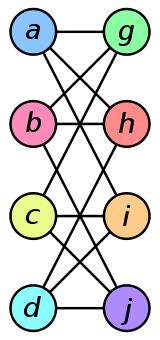
\includegraphics[scale=0.3]{graph-iso-a}
        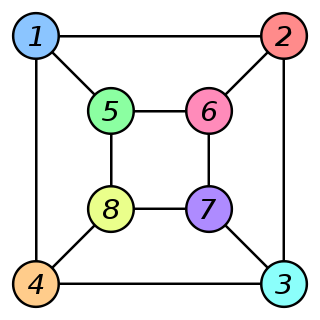
\includegraphics[scale=0.3]{graph-iso-b}
    \end{figure}

    There also exists the \textit{Subgraph Isomorphism} problems: given $G_1$ and $G_2$,
    determine if $G_2$ is a subgraph of $G_1$. However, Subgraph Isomorphism, which is definitively NP-complete~\cite{cook1971complexity},
    is a generalization of Graph Isomorphism, so we won't consider this in the same problem set as Graph Isomorphism.
    \\
    However, it should be noted that determining
    Graph Isomorphism is complex in its own right. In fact, determining graph isomorphism falls
    into its own category of problem complexity, called \textit{Graph Isomorphism Complete}.
    According to Lubiw, it has yet to fall into a typical classification, and is neither P nor NP-complete~\cite{anna-complexity}.
    There exists no known P algorithm, yet graph isomorphism has not been shown to be NP-complete. This means that either a P algorithm
    must exist for graph isomorphism but is undiscovered, graph isomorhpism is a problem outside of
    P and NP, or, as Schöning argues, Graph isomorphism problems are in the low hierarchy of NP,
    which "does not equal NP unless the polynomial hierarchy collapses to the second level"~\cite{np-hierarchy}.
    Deeper explanation of this exceeds the reaches of this paper.
    \\
    \\
    While there is really just one representative problem of this class - determine if two graphs are isomorphic -
    there are a large variety of consequential applications to solving this problem. For instance,
    database searches that use graphs instead of keywords. A great example of this is the biochemical search
    engine described by Bonnici et al.; Given unknown "biological networks at the molecular, protein, or species level",
    in a graph representation, how can we determine if it subject already exists in current records?
    We can perform a graph isomorphism against the database of graphs of existing subjects
    to determine if our unknown subject has previously been discovered and other relevant information.
    Because this is such an expensive process, it would make sense to filter results on other criteria
    before determining graph isomorphism, or to use graph isomorphism algorithms to eliminate matches
    as quickly as possible to reduce the search space ~\cite{Bonnici2013}.
    \\
    Other applications exist in automata (comparing languages), social networks, chemical structure analysis,
    and image processing.
    \\\\
    The best currently accepted theoretical algorithm belongs to Lazlo Babai and Eugene Luks~\cite{BabaiLuksGoodAlgorithm}.
    The algorithm relies on canonical labelling of the graphs. A basic algorithm that uses canonical
    labelling for graph isomorphism would be as follows.\\\\
    Given two finite graphs with unknown isomorphism $G_1$ and $G_2$ where $|G_1.V| = |G_2.V|$, assign a count label $v.c$
    that is the outdegree for every vertex in $G_1$ and $G_2$. First, check that the frequency of all
    outdegrees are the same for both graphs (if it isn't, they are not isomorphic). Then,
    starting with the outdegree of lowest frequency
    select vertices $v_1 \in G_1.V$ and $v_2 \in G_2.V$ with the same outdegrees.
    Perform a simultaneous BFS on $G_1$ and $G_2$ starting from $v_1$ and $v_2$, comparing the
    outdegrees of all of the neighoring vertices. If ever the neghboring outdegrees of $v_1$ and $v_2$ don't match, try a different pair
    of start vertices $v_1$ and $v_2$ until you have exhausted all vertices of that outdegree (at which point we
    can say that $G_1$ and $G_2$ are not isomorphic). If all outdegrees match for a certain combination $v_1, v_2$, continue this process
    for the remaining unvisitied vertices until both graphs are fully visited or $G_1$ and $G_2$ are
    found to not be isomorphic. If you can visit all vertices in $G_1$ and $G_2$ and match all $v.c$ in $G_1$
    and $G_2$, we can consider them isomorphic.
    \\\\ Often, graphs that have more meaningful labels on their vertices
    can be more easily determined as isomorphic or not because more unique information can be used to
    more quickly filter out incorrect adjacent vertices.


\pagebreak
\bibliography{mybib}{}
\bibliographystyle{abbrv}
\end{document}
